\documentclass{article}
\usepackage{graphicx}
\usepackage{url}
\graphicspath{/home/shriya/tex document/}
\title{Assignment 4}
\author{Shriya Shukla}
\begin{document}
\section{Shriya Shukla (ME20B163)}
\subsection{Bernoulli's Equation} \cite{bernoullieq}
\begin{equation}
P_{1}+\frac{1}{2}\rho v_{1}^{2}+\rho g h_{1}=P_{2}+\frac{1}{2}\rho v_{2}^{2}+\rho g h_{2}=constant \label{eq.1} 
\end{equation}

\begin{flushleft}
$\rho$ = fluid density \newline
$P_{1}$=pressure at elevation 1 \\
$g$= acceleration due to gravity \\
$v_{1}$	=velocity at elevation 1 \\
$h_{1}$	=height of elevation 1 \\
$P_{2}$	=pressure at elevation 2 \\
$v_{2}$	=velocity at elevation 2 \\
$h_{2}$	=height at elevation 2 \\

\end{flushleft}
\paragraph{}
In fluid dynamics, Bernoulli's principle states that an increase in speed of the fluid occurs simultaneously with decrease in static pressure or decrease in the fluid's potential energy. The above Bernoulli's equation \ref{eq.1} was derived by Leonhard Euler. A better visual explanation of the equation is given in figure \ref{fig:bernoulli}
\begin{figure}[h]
\begin{center}

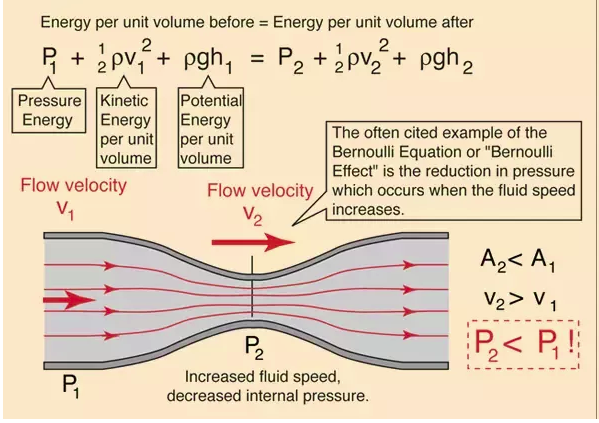
\includegraphics[width=200px]{ME20B163.png} 
\caption{ME20B163}\cite{ME20B163}
\label{fig:bernoulli}		
		 
\end{center}
\end{figure}

\bibliography{ME20B163.bib}
\bibliographystyle{plain}

\end{document}